\chapter{Results}
\label{cha:Results}
In this section, we will give some examples of generated reports obtained by passing a full program as input to the type extractor. The program analysis is not supposed to be fast. The overhead of a Lua call for each hook is high enough to leverage time performance. In this section we will present some reports generated by the extractor when analysing simple Lua programs and also Lua benchmark programs.

\section*{Basic}
A basic functionality of the extractor is represented by the Image~\ref{fig:basic1}. The output generated is related to the execution of Code~\ref{basic1}.
\lstinputlisting[label=basic1,title={Basic example 1},caption={Basic example 1}, language={[5.0]Lua}]{codes/basic_1.lua}

Image~\ref{fig:basic2} shows the output for Code~\ref{basic2}.
\lstinputlisting[label=basic2,title={Basic example 2},caption={Basic example 2}, language={[5.0]Lua}]{codes/basic_2.lua}

\begin{figure}
    \centering
    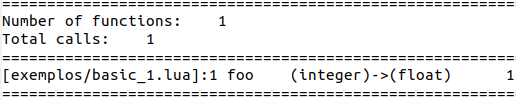
\includegraphics[width=0.85\textwidth]{pictures/basic1.png}
    \caption{Basic example 1}
    \label{fig:basic1}
    \end{figure}
\section*{}
% \lstinputlisting[label=mean2,title={Mean Filter},caption={Mean Filter},language=R]{codes/mean.R}